% !TEX program = xelatex
\documentclass[11pt,aspectratio=169]{beamer}

\makeatletter
\def\@makefnmark{}
\makeatletter

\setbeamersize{text margin left=5mm,text margin right=5mm} 

\usepackage{amsthm,amsmath,amssymb,braket,fontspec,unicode-math}
\usepackage[absolute,overlay]{textpos}

\usetheme[numbering=none,nofirafonts]{focus}

\setbeamercolor{footnote}{fg=blue}
\setbeamerfont{footnote}{size=\small}
\setbeamertemplate{bibliography item}[triangle]

\setmainfont{FiraCode Nerd Font}
\setsansfont{Fira Sans}
\setmathfont{Fira Math}
\setbeamerfont{title}{size=\LARGE, shape=\scshape}
\setbeamerfont{author}{size=\large, shape=\scshape}
\setbeamerfont{institute}{size=\normalsize, shape=\scshape}
\setbeamerfont{date}{size=\normalsize, shape=\scshape}
\setbeamerfont{frametitle}{size=\large, shape=\scshape}

\usepackage[backend=bibtex,url=false,doi=false,maxcitenames=1, style=authoryear]{biblatex}
\bibliography{bib}
\AtBeginBibliography{\scriptsize}

\newcommand{\focus}[1]{\textcolor{red}{#1}}

\definecolor{red}{HTML}{CC0000}
\setbeamertemplate{bibliography item}[triangle]

\AtBeginSection[]{
\begin{frame}
  \vfill
  \centering
  \begin{beamercolorbox}[sep=20pt,rounded=true,center]{frametitle}
    \usebeamerfont{title}\insertsectionhead\par%
  \end{beamercolorbox}
  \vfill
\end{frame}
}
\title{
{Hierarchical structure and topological content of entanglement of free fermions}
}
\date{\today}
\author{Abhirup Mukherjee, Siddhartha Patra, Siddhartha Lal}
\institute{Department of Physical Sciences, IISER Kolkata, Mohanpur}
\date{\today}

\begin{document}

\centering

\begin{frame}
\maketitle
\begin{textblock*}{0.4\textwidth}(5.5cm, 6.5cm)
	\centering
	\vspace*{\fill}

	
\includegraphics[width=0.35\textwidth]{figures/epqm_logo_mod.jpeg}
	\hspace*{\fill}
	
\includegraphics[width=0.35\textwidth]{figures/dps_logo.jpeg}

	\vspace*{\fill}
\end{textblock*}
\end{frame}

\section{Introduction}

\begin{frame}{The system}

{Massless Dirac fermions on a 2-torus}
\[\mathcal{L} = i\overline\psi\gamma_\mu\partial_\mu \psi\]
{In presence of an Aharonov-Bohm flux}
\[\mathcal{L} = \overline\psi \left(i\gamma_\mu + eA_\mu\right)\partial_\mu \psi\]
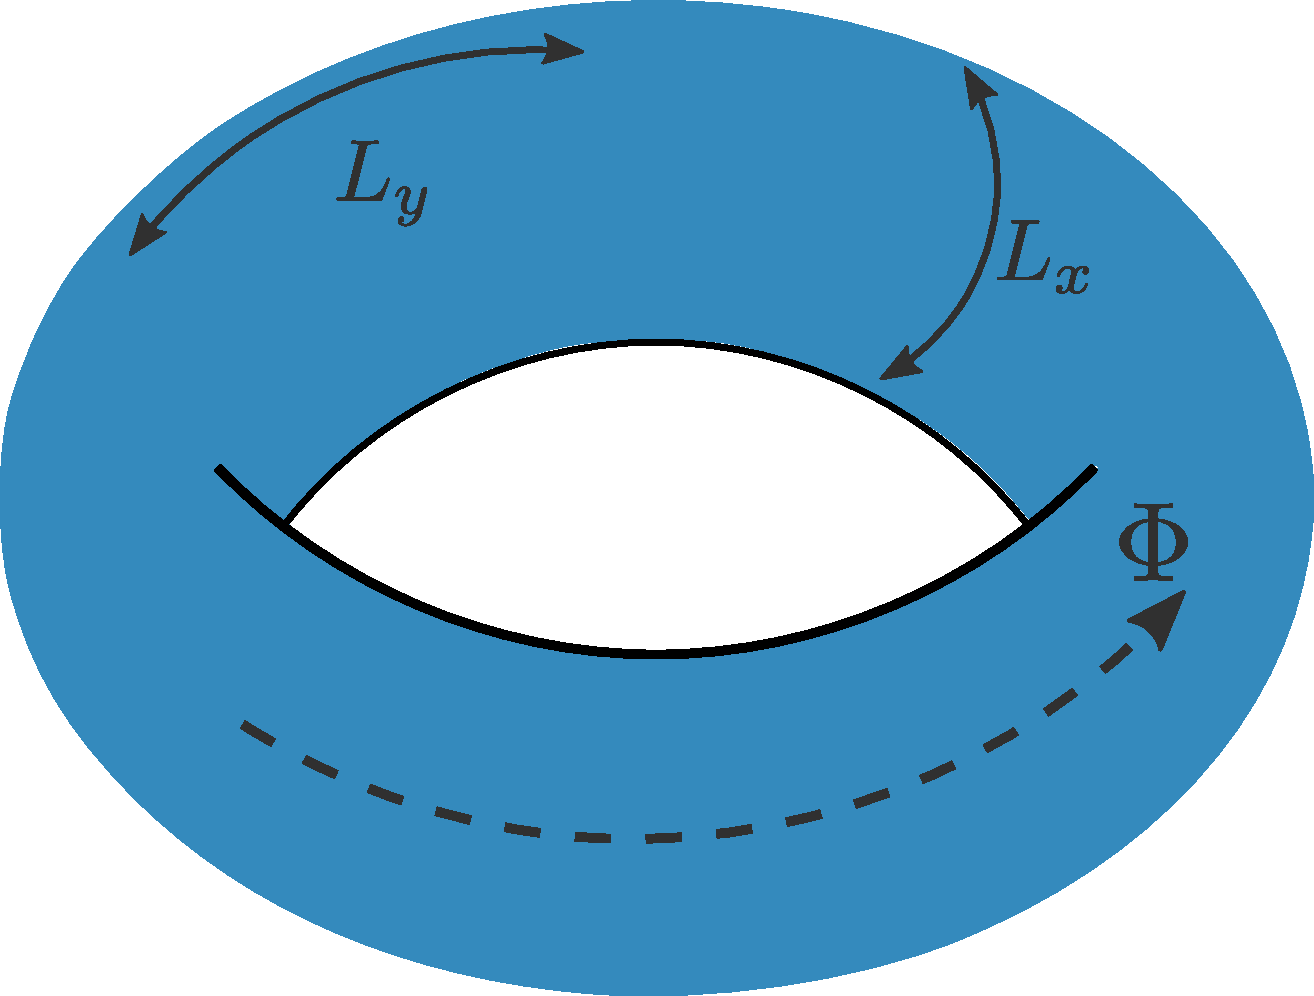
\includegraphics[width=0.4\textwidth]{figures/torus.pdf}
\hspace*{\fill}
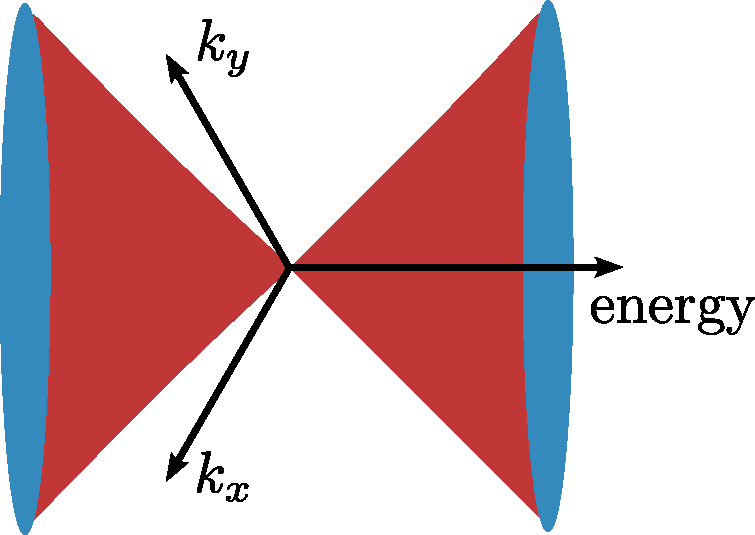
\includegraphics[width=0.42\textwidth]{figures/dirac.pdf}

\end{frame}

\begin{frame}{Measures of entanglement}
\vspace*{-30pt}
	\begin{minipage}{0.39\textwidth}
	\vspace*{30pt}
	\only<1-4>{
	\(\rho = \ket{\Psi}\bra{\Psi}\longrightarrow\)\focus{density matrix}\\[20pt]
	\only<2->{\(\rho_A = \) partial trace over system A\\
	\(\longrightarrow\) \focus{reduced DM}\\[20pt]}
}
	\end{minipage}
	\hspace*{10pt}
	\begin{minipage}{0.55\textwidth}
		\centering
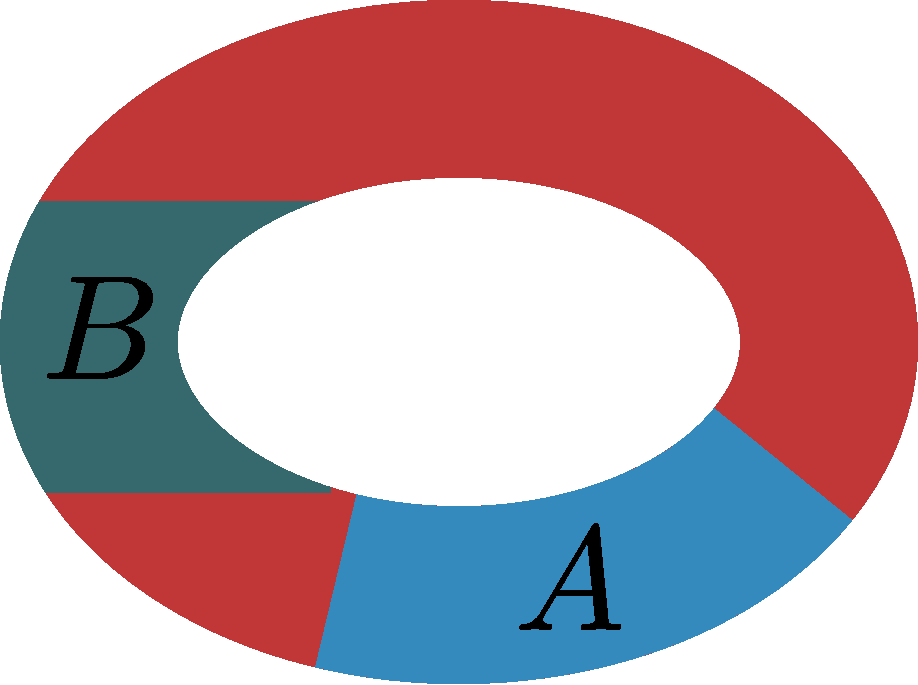
\includegraphics[width=0.49\textwidth]{figures/subsystem-A.pdf}
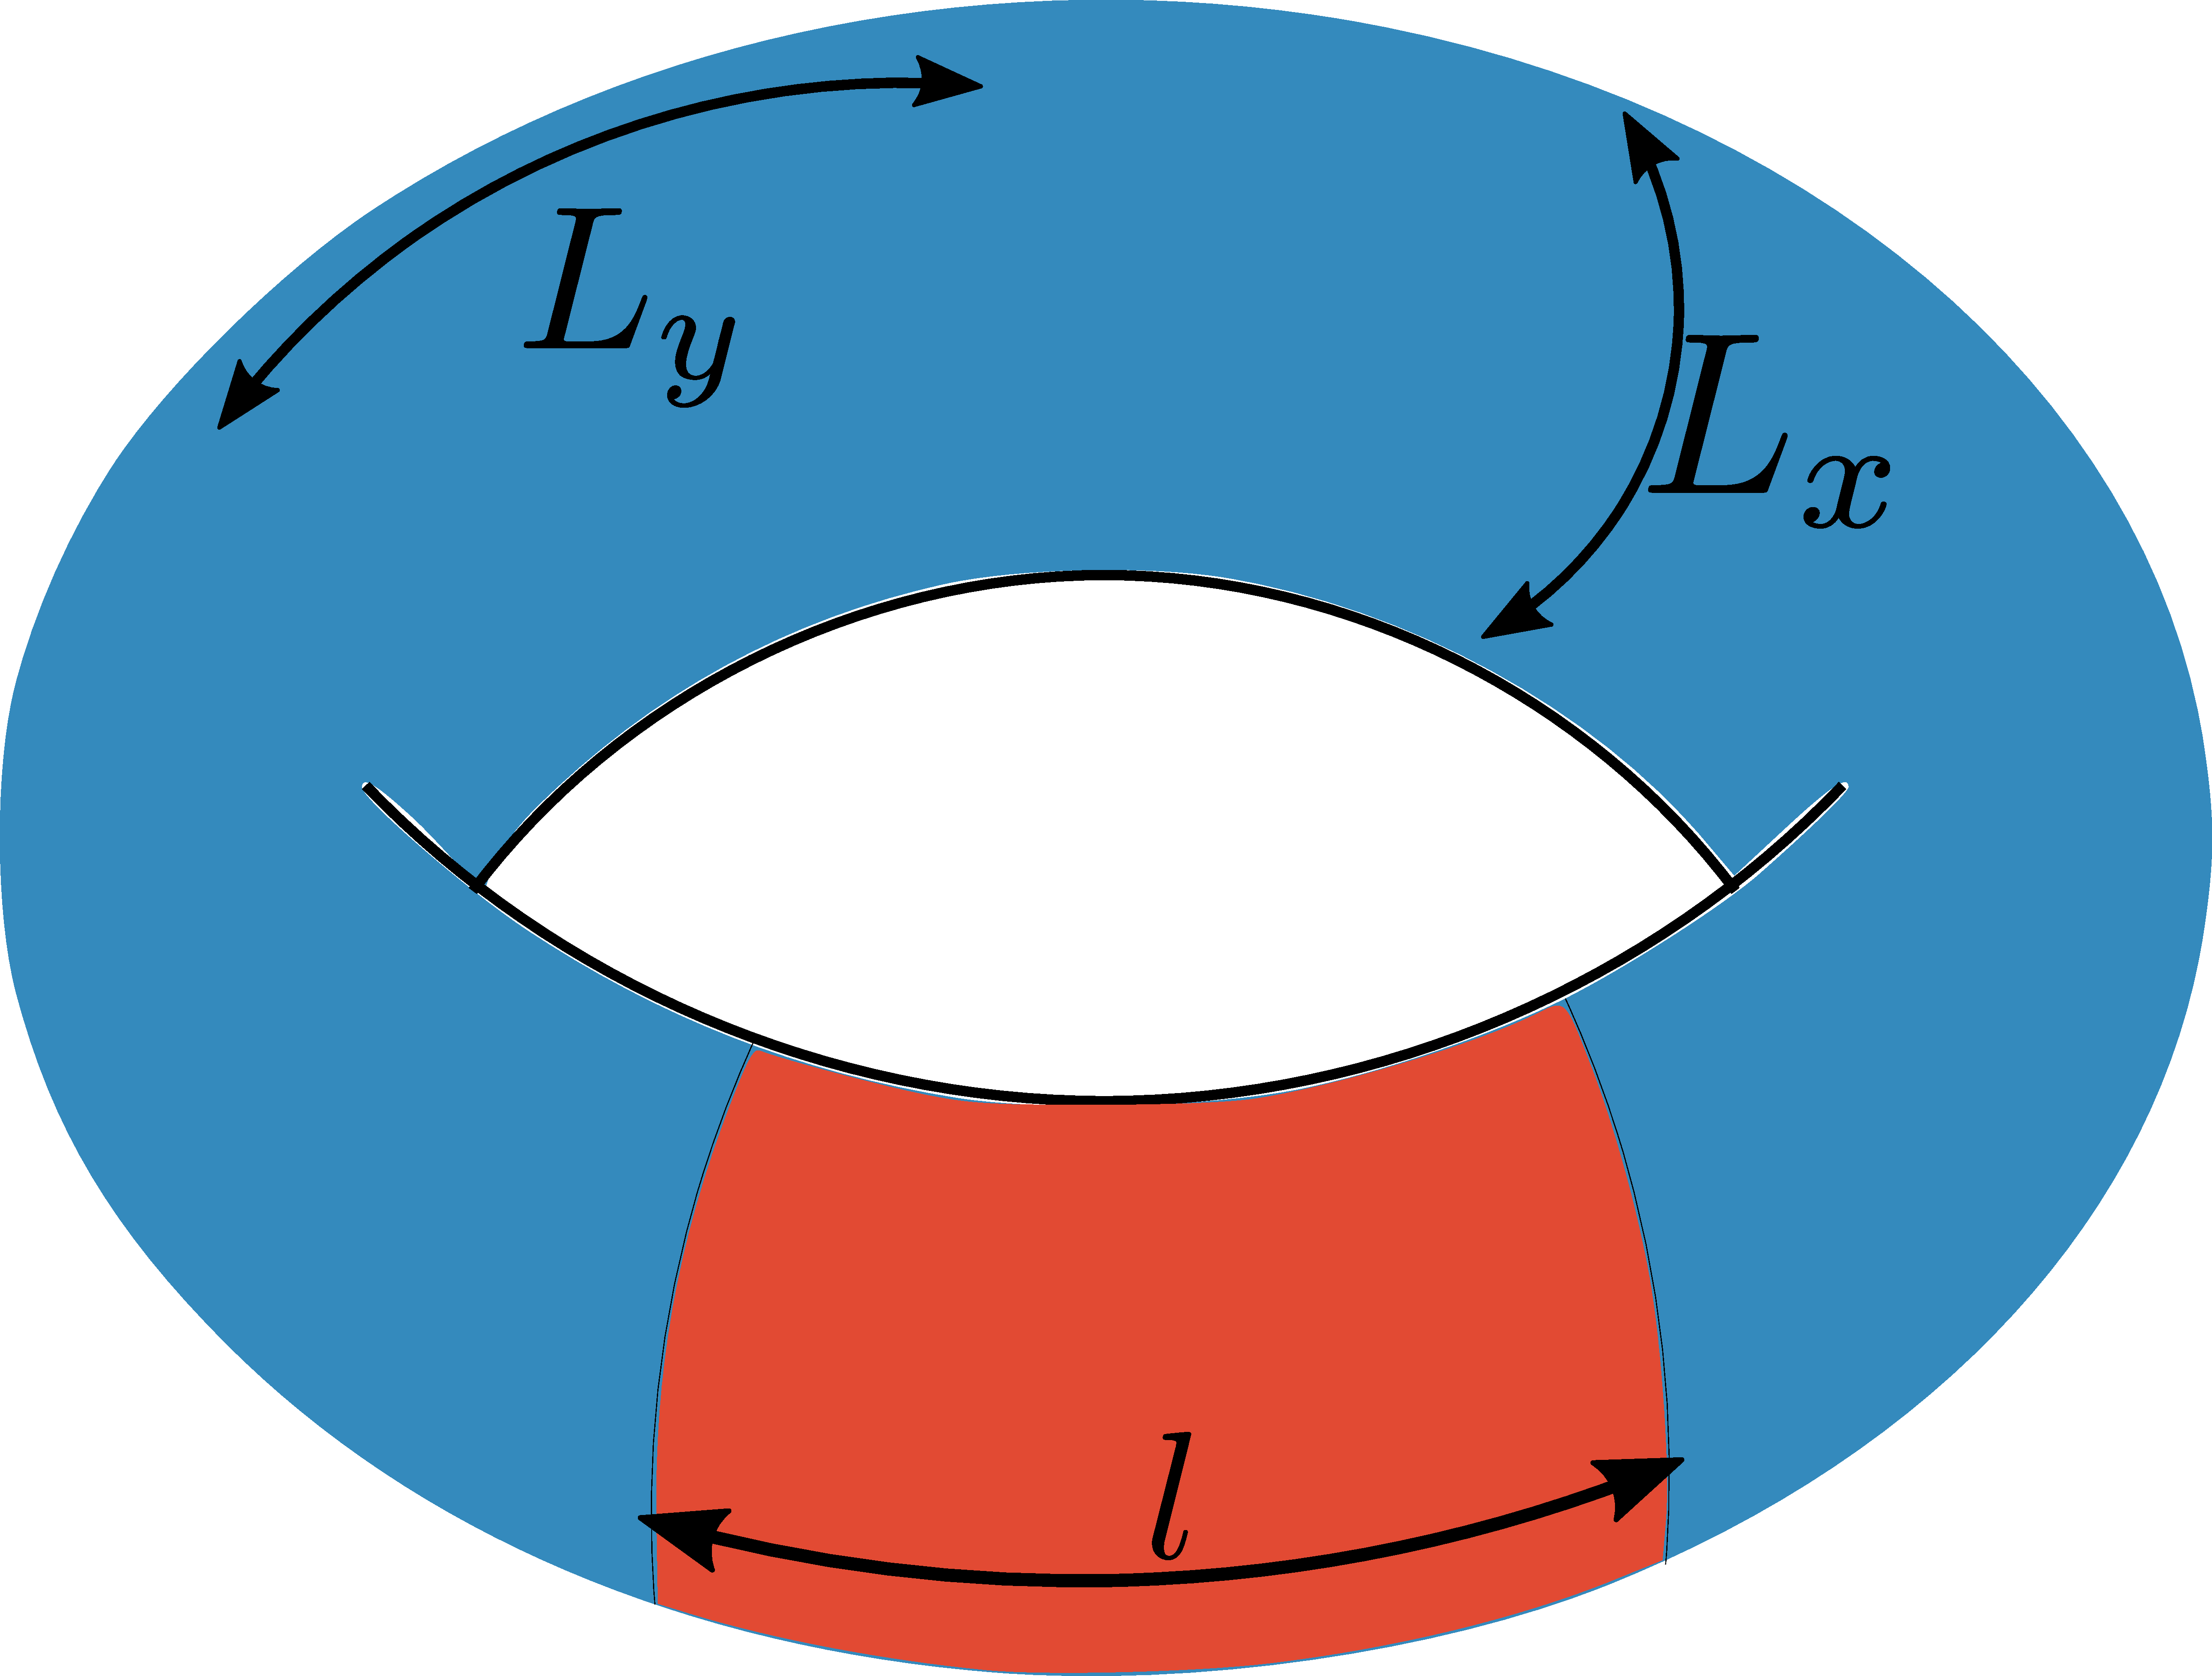
\includegraphics[width=0.49\textwidth]{figures/subsystem-torus.pdf}
\end{minipage}

\vspace*{\fill}

\only<3>{\(S(A) = -\text{Tr}\left[\rho_A \ln \rho_A\right] \longrightarrow\) \focus{entanglement entropy} of A\\[10pt]
\(\longrightarrow\) quantifies information shared between \(A\) and rest}
	\only<4>{\(I(A:B) = S(A) + S(B) - S(A \cup B) \longrightarrow\) \focus{mutual information} between \(A\) and \(B\)\\[10pt]
\(\longrightarrow\) quantifies information shared between \(A\) and \(B\)}
\end{frame}

\begin{frame}{Entanglement of free fermions}
	Diagonal in \(k-\)space \(\mathbf\longrightarrow\) \focus{Vanishing} entanglement in momentum space\\[20pt]
	\only<2>{Off-diagonal in \(r-\)space \(\mathbf\longrightarrow\) \focus{Fluctuations} exist in real space\\
		\(\mathbf\longrightarrow\) leads to entanglement in real space\\[20pt]
	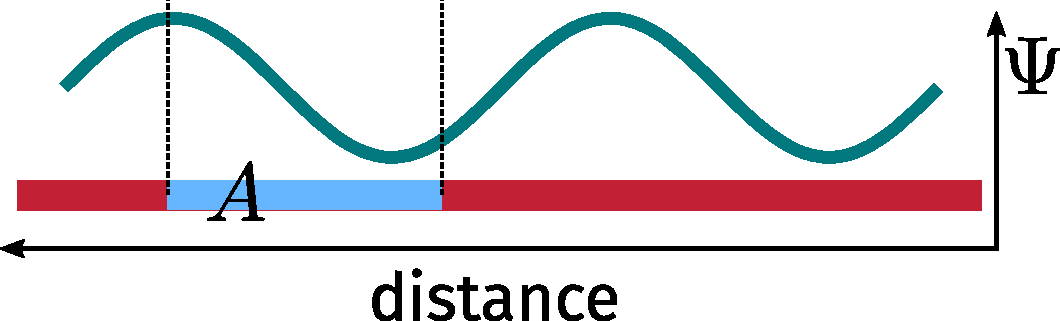
\includegraphics[width=0.6\textwidth]{figures/nonlocal.pdf}}
\end{frame}

\begin{frame}{Entanglement of free fermions}
	\begin{minipage}{0.6\textwidth}
		\vspace{15pt}
	\(1D\)-ring of massless fermions: \(~ ~ ~ ~ \frac{2}{3} \ln \left( \frac{L}{\pi a} \sin \frac{\pi l}{L}\right) \)
		\vspace{15pt}
	\end{minipage}
	\begin{minipage}{0.39\textwidth}
		\centering
		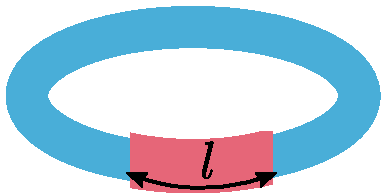
\includegraphics[width=0.8\textwidth]{figures/ring.pdf}
	\end{minipage}

	\begin{minipage}{0.6\textwidth}
		\vspace{15pt}
	\(1D\)-line of massless fermions: \(~ ~ ~ ~ \frac{1}{3} \ln \left( \frac{2L}{\pi a} \sin \frac{\pi l}{L}\right) \)
		\vspace{15pt}
	\end{minipage}
	\begin{minipage}{0.39\textwidth}
		\centering
		
\includegraphics[width=\textwidth]{figures/open.pdf}
	\end{minipage}

	\begin{minipage}{0.6\textwidth}
		\vspace{15pt}
	\(1D\)-line of relativistic fermions: \(~ ~ ~ ~ -\frac{1}{3} \ln \left( m a\right) \)
		\vspace{15pt}
	\end{minipage}
	\begin{minipage}{0.39\textwidth}
		\centering
		
\includegraphics[width=\textwidth]{figures/open.pdf}
	\end{minipage}

	\begin{minipage}{0.6\textwidth}
	\vspace{15pt}
	\(2D\)-torus of massless fermions: \(~ ~ ~ ~ \alpha \frac{L_y}{\epsilon} \)\\
	\end{minipage}
	\begin{minipage}{0.39\textwidth}
		\centering
		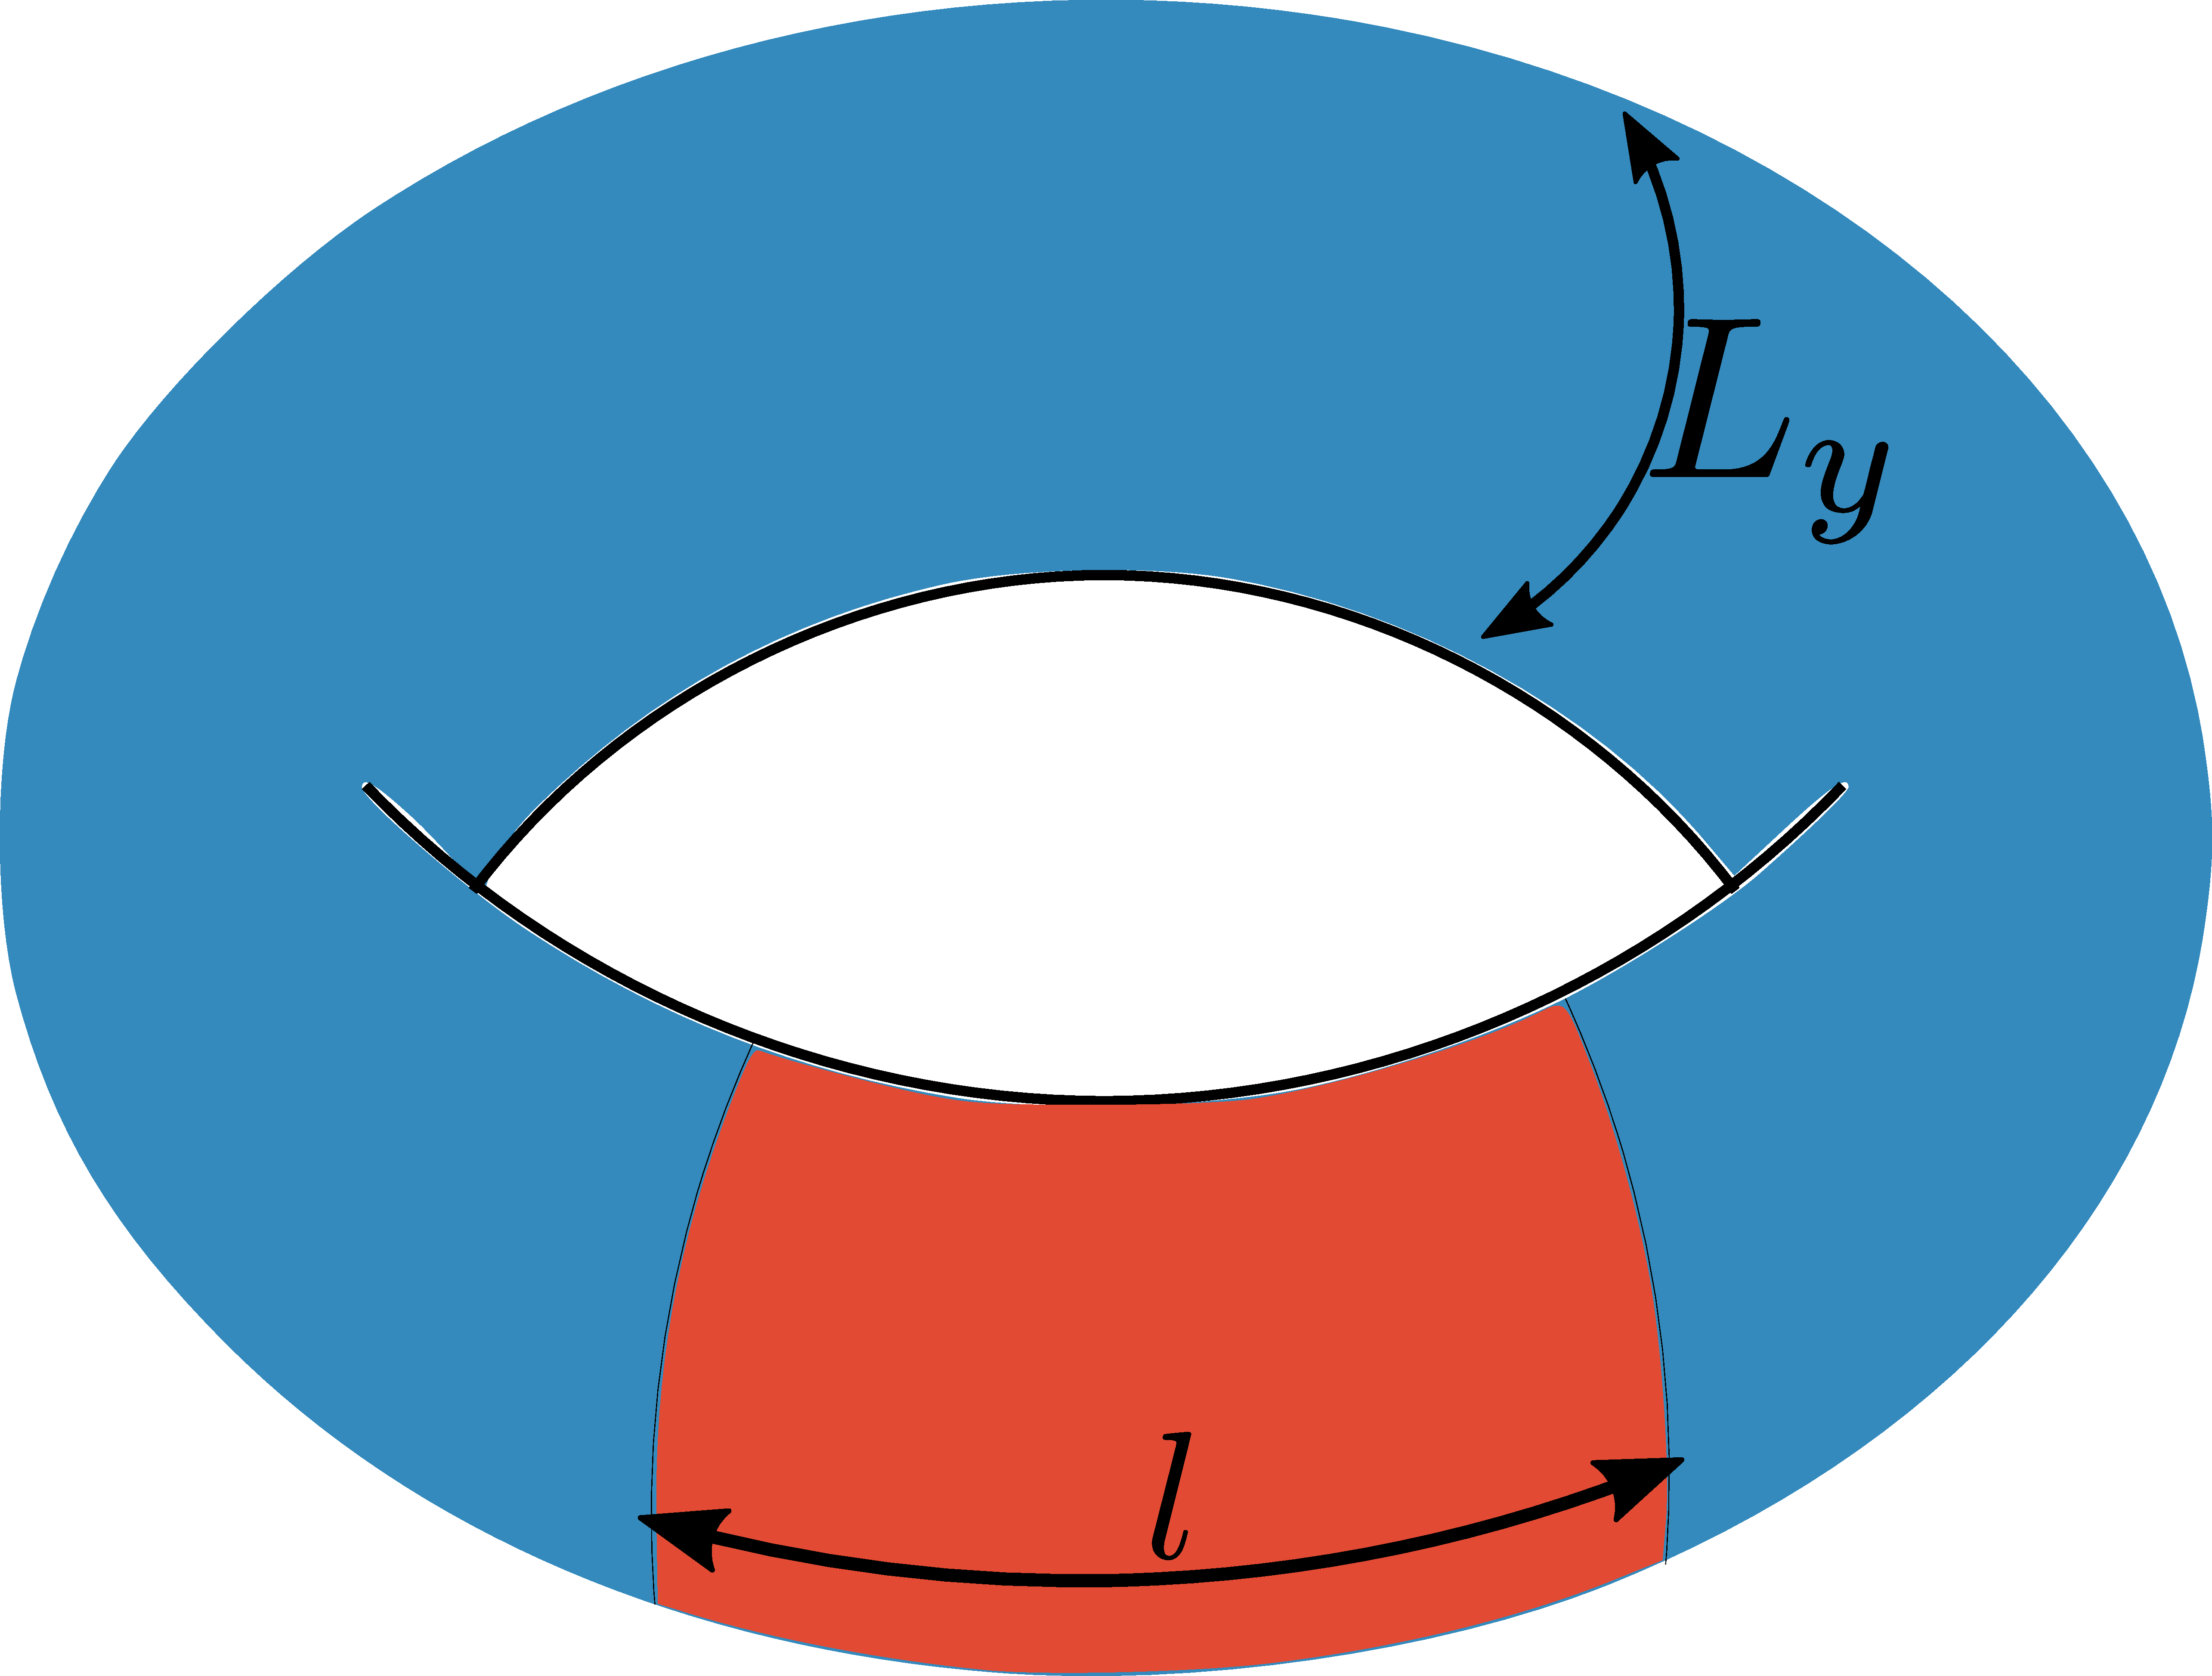
\includegraphics[width=0.5\textwidth]{figures/torus-EE.pdf}
	\end{minipage}
\end{frame}

\section{What are we going after?}

\begin{frame}{What are we going after?}
	\begin{itemize}
		\item Effect of a magnetic flux on the entanglement\\[20pt]
		\item Distribution of the entanglement among subsystems of various sizes\\[20pt]
		\item Emergent space generated by the transformations between these subsystems\\[20pt]
		\item Curvature and related quantities of this space
	\end{itemize}

\end{frame}

\section{Reduction to \(1+1-\)D systems}

\begin{frame}{Reduction to \(1+1-\)D systems}
\vspace*{20pt}
	\only<1>{In presence of flux: ~ ~ ~{\Large\(\mathcal{L} = \int dx dy ~ ~ ~\overline\Psi(x) \left(i\gamma_\mu + eA_\mu\right)\partial_\mu \Psi(x)\)}\\[20pt]
	Periodic boundary conditions along \(\vec x\): ~ ~ ~ {\Large \(k_x^n = \frac{2\pi n }{L_x},~ ~ n \in \mathbb{Z} \)}\\[20pt]
	Introduce Fourier modes: ~ ~ ~ {\Large \(\Psi(x) = \sum_{n=-\infty}^\infty e^{i x k_x^n}\Psi(k_x^n)\)}
}
\only<2>{
Decouples into \(1D\) modes: ~ ~ {\Large \(\mathcal{L}=\sum_{n} \int dy ~ \overline\Psi(k_x,y) \left(i\gamma_\mu \partial_\mu - M\right) \Psi(k_x, y)\)}\\

\vspace*{20pt}

\includegraphics[width=0.7\textwidth]{figures/dim-reduc.pdf}
}
\only<3>{
	\(2D\) system is described by sum over \(1D\) modes.\\[10pt]
	{\LARGE\(\downarrow\)}\\[10pt]
	Modes do not couple - no inter-mode entanglement.\\[10pt]
	{\LARGE\(\downarrow\)}\\[10pt]
Total entanglement is sum of each part: ~ {\Large\(S = \sum_n S_n\)}\\[10pt]
\[S_n(\phi) =- c \ln \left(\epsilon \frac{2\pi |n+\phi|}{L_x}\right) \]
}
\end{frame}

\begin{frame}[allowframebreaks]{References}
\printbibliography
\end{frame}

\end{document}
